\documentclass[11pt,a4paper,oneside]{book}

% -----------------------------------------------------------------------------
% Packages
% -----------------------------------------------------------------------------
\usepackage[a4paper, top=1in, bottom=1in, left=1in, right=1in, headheight=14.5pt]{geometry}
\usepackage{amsmath,amssymb}
\usepackage{graphicx}
\graphicspath{{../}{./}}
\usepackage{booktabs}
\usepackage{fancyhdr}
\usepackage{titlesec}
\usepackage{cite}
\usepackage{tabularx}
\usepackage{array}
\usepackage{float}
\usepackage{xcolor}
\usepackage{hyperref}

% -----------------------------------------------------------------------------
% Hyperlink & Metadata Configuration
% -----------------------------------------------------------------------------
\hypersetup{
    colorlinks=true,
    linkcolor=black,
    citecolor=blue!70!black,
    urlcolor=blue!70!black,
    plainpages=false,
    pdftitle={A Comparative Analysis of Cryptographic Primitives in Blockchains},
    pdfauthor={Group 2}
}

% -----------------------------------------------------------------------------
% Typography & Page Breaking Adjustments
% -----------------------------------------------------------------------------
\renewcommand{\baselinestretch}{1.10}
\setlength{\parskip}{0.3em}
\setlength{\parindent}{0pt}

\raggedbottom
\clubpenalty=10000
\widowpenalty=10000
\displaywidowpenalty=10000

\renewcommand{\bibname}{References}

% Chapter & Section Headings 
\titleformat{\chapter}[hang]{\huge\bfseries}{\thechapter.}{0.5em}{}
\titlespacing*{\chapter}{0pt}{0pt}{15pt}
\titleformat{\section}{\Large\bfseries}{\thesection}{0.5em}{}
\titleformat{\subsection}{\large\bfseries}{\thesubsection}{0.5em}{}

% -----------------------------------------------------------------------------
% Header & Footer 
% -----------------------------------------------------------------------------
\pagestyle{fancy}
\fancyhf{}
\fancyhead[L]{\small BITS F463: Cryptography}
\fancyhead[C]{\small Midsem Assignment Report}
\fancyhead[R]{\small Group 2}
\fancyfoot[C]{\thepage}
\renewcommand{\headrulewidth}{0.4pt}

\fancypagestyle{plain}{
    \fancyhf{}
    \fancyhead[L]{\small BITS F463: Cryptography}
    \fancyhead[C]{\small Midsem Assignment Report}
    \fancyhead[R]{\small Group 2}
    \fancyfoot[C]{\thepage}
    \renewcommand{\headrulewidth}{0.4pt}
}

% -----------------------------------------------------------------------------
% Document Start
% -----------------------------------------------------------------------------
\begin{document}

\hypersetup{pageanchor=false}
\begin{titlepage}
    \vspace*{1.5in}

    \begin{center}
        {\Huge \textbf{A Comparative Analysis of Cryptographic Primitives in Blockchains}} \\[1.5in]

        {\Large \textbf{BITS F463: Cryptography}} \\[0.3em]
        {\Large Midsem Assignment Report} \\[1.5in]

        {\Large \textbf{Group 2}} \\[0.8em]
        {\large Shaurya Suman (2024A7PS0589G)} \\[0.3em]
        {\large Tushar Kumar (2024A7PS0477G)}
    \end{center}

    \vfill

    \begin{center}
        {\large \textbf{Birla Institute of Technology \& Science, Pilani}} \\[0.2em]
        {\large \textbf{K. K. Birla Goa Campus}}
    \end{center}
\end{titlepage}
\hypersetup{pageanchor=true}

\frontmatter
\tableofcontents
\newpage

\mainmatter

\chapter{Introduction}

Modern decentralized ledgers operate without a central authority or trusted third party. To maintain trust, they depend entirely on two foundational cryptographic pillars:
\begin{enumerate}
    \item \textbf{Hash Functions:} These act as the network's mathematical glue. They ensure transaction data has not been tampered with, chain blocks together to form an immutable history, and often serve as the puzzle mechanism for consensus (like mining).
    \item \textbf{Digital Signature Schemes:} These act as digital fingerprints, providing authentication and non-repudiation so that only the true owner of a digital asset can authorize its transfer.
\end{enumerate}

A common misconception is that a hash function is just a generic "black box" that securely scrambles data, and that any modern algorithm will work equally well for any blockchain. In reality, the \textit{internal mechanics} of a hash function dictate the economic and security reality of the entire network.

Different blockchains have entirely different goals, and thus, they deliberately choose hash functions with different structural trade-offs. For example, Bitcoin uses SHA-256, an algorithm that is computationally simple~\cite{nakamoto2008bitcoin}. Because it is simple, specialized hardware companies can manufacture chips (ASICs) that do nothing but calculate SHA-256 billions of times per second. This secures the network but leads to massive mining centralization. Litecoin, wanting to keep mining accessible to regular users, chose Scrypt---an algorithm specifically designed to bottleneck the computer's memory, making those specialized ASIC chips economically unviable to produce~\cite{percival2009scrypt}. Similarly, Ethereum adopted Sponge constructions (Keccak-256) to eliminate specific mathematical vulnerabilities entirely~\cite{wood2014ethereum}.

The overarching objective of this assignment is to bridge the gap between cryptographic theory and real-world execution. We will take the theoretical claims made about these different algorithms---such as "Scrypt consumes excessive memory" or "BLAKE2b is faster in software"---and test them empirically. By building an isolated test harness and running these algorithms on standard consumer hardware, we aim to measure exactly how these distinct mathematical architectures perform in practice regarding speed, memory utilization, and security properties.


\chapter{Literature Survey}

\section{Selection Rationale}
To capture the full spectrum of how blockchains balance security, speed, and decentralization, we selected four algorithms representing fundamentally distinct mathematical architectures. Each was chosen to solve a specific problem in distributed systems:
\begin{itemize}
    \item \textbf{SHA-256 (Merkle-Damg{\aa}rd):} Selected as the historical baseline. It prioritizes pure computational predictability and is the backbone of Bitcoin.
    \item \textbf{Keccak-256 / SHA3-256 (Sponge):} Selected for its advanced security. Ethereum chose this to eliminate specific structural vulnerabilities present in older hashes.
    \item \textbf{Scrypt (Memory-Hard PBKDF):} Selected for its economic impact. It was designed to resist hardware centralization by forcing the computer to consume large amounts of RAM.
    \item \textbf{BLAKE2b (ARX):} Selected for raw speed. It is engineered to be blazingly fast on standard consumer laptops and desktops, favored by modern Proof-of-Stake networks.
\end{itemize}

\section{SHA-256 (Merkle-Damg{\aa}rd Architecture)}
Employed by Bitcoin, SHA-256 operates on the classic Merkle-Damg{\aa}rd iterative construction~\cite{nakamoto2008bitcoin, schneier1996applied}. The input message is padded, chopped into 512-bit blocks, and processed one by one. The algorithm uses elementary operations: 32-bit addition, shifting bits, and XORing.

Because it only uses these basic math operations and requires almost zero working memory, it is incredibly easy to hardwire into custom silicon. This is why Application-Specific Integrated Circuits (ASICs) exist for Bitcoin: factories print chips that cannot run an operating system or play a game, but can execute SHA-256 math millions of times faster than a standard CPU. While this provides massive network security, it prices normal users out of the mining process. Furthermore, the block-by-block nature of this architecture leaves it vulnerable to "length-extension attacks" (where an attacker can append data to a hash without knowing the original input), which is why Bitcoin hashes everything twice: $\text{SHA-256}(\text{SHA-256}(m))$.

\section{Keccak-256 / SHA3-256 (Sponge Construction)}
To avoid the vulnerabilities of older hashes, Ethereum selected Keccak-256, which uses a "Sponge" construction~\cite{wood2014ethereum, bertoni2013keccak}. Instead of compressing blocks one by one, Keccak maintains a massive 1600-bit internal state. It "absorbs" the input data into a portion of this state, completely scrambles the entire 1600 bits using a complex 24-round permutation function, and then "squeezes" out the final hash.

Because a large portion of this internal state (the "capacity") is never exposed to the outside world, attackers cannot reverse-engineer the state to perform length-extension attacks. The trade-off is speed: manipulating a 1600-bit state in pure software requires significantly more computational effort than SHA-256~\cite{paar2024understanding}.

\section{Scrypt (Memory-Hard Key Derivation)}
Developed by Colin Percival and popularized by Litecoin, Scrypt is not a traditional hash; it is a password-based key derivation function explicitly designed to be "memory-hard"~\cite{percival2009scrypt}.

To prevent the ASIC centralization seen in Bitcoin, Scrypt attacks the hardware supply chain. While it is cheap to put thousands of math-calculating cores on a silicon chip, physical RAM is extremely expensive and takes up physical space. Scrypt forces the computer to sequentially generate a massive array of pseudo-random data in RAM, and then randomly read from that array to calculate the final hash. If a specialized mining chip tries to bypass storing this data to save money on RAM, the mathematical penalty forces the chip to recalculate the data from scratch, completely destroying its speed advantage. This intentional memory bottleneck keeps mining accessible to consumer GPUs and CPUs.

\section{BLAKE2b (ARX Architecture)}
Standardized under RFC 7693 and used by networks like Cardano and Polkadot, BLAKE2b is built on an Addition-Rotation-XOR (ARX) architecture~\cite{aumasson2013blake2}.

Unlike older algorithms that rely on complex mathematical mixing, ARX algorithms rely only on adding, rotating, and XORing binary numbers. These happen to be the three operations that modern 64-bit consumer processors (like those in normal laptops) can execute faster than anything else. BLAKE2b was meticulously optimized to leverage the native architecture of everyday computers, making it theoretically faster than any other cryptographic hash in pure software execution.

\section{Architectural Summary}
Table~\ref{tab:lit_comparison} synthesizes the conceptual trade-offs among the four target primitives before we put them to the test in our empirical benchmarking.

\begin{table}[H]
    \centering
    \caption{Conceptual Comparison of Target Cryptographic Hashing Primitives}
    \label{tab:lit_comparison}
    \vspace{0.4em}
    \small
    \begin{tabularx}{\textwidth}{@{}l l l >{\raggedright\arraybackslash}X >{\raggedright\arraybackslash}X@{}}
        \toprule
        \textbf{Algorithm} & \textbf{Dominant Network} & \textbf{Core Architecture} & \textbf{Primary Design Focus}  & \textbf{Hardware Orientation} \\
        \midrule
        SHA-256            & Bitcoin                   & Merkle-Damg{\aa}rd         & Computational predictability   & Custom silicon (ASIC-leaning) \\
        Keccak-256         & Ethereum                  & Sponge Construction        & Length-extension immunity      & Balanced / Silicon-friendly   \\
        Scrypt             & Litecoin                  & Memory-Hard PBKDF          & ASIC resistance / memory bound & System memory (RAM-bound)     \\
        BLAKE2b            & Cardano/Polkadot          & ARX (ChaCha core)          & 64-bit software throughput     & Commodity 64-bit CPUs         \\
        \bottomrule
    \end{tabularx}
\end{table}


\chapter{Plan of Action}

Our goal is to write a software suite that puts these theoretical claims to the test. The assignment roadmap is structured into two sequential phases aligned with the course milestones.

\section{Phase 1: Hash Functions}
Phase 1 focuses entirely on the data integrity pillar. We will benchmark hash primitives through the following structured steps:
\begin{itemize}
    \item \textbf{Step 1: Test Harness Construction:} We will build a reproducible Python testing suite using raw cryptographic bindings via Python's native \texttt{hashlib} and platform-native libraries. This allows us to measure pure algorithmic execution in the underlying C/C++ backends without Python object overhead.

    \item \textbf{Step 2: Avalanche Effect Verification:} A good hash function must look completely random. If we flip a single binary bit in the input file, roughly 50\% of the output bits should flip. We mathematically test this by XORing the original and modified digests to calculate the Hamming distance ($H$), defined as:
          $$ \text{Avalanche Ratio} = \frac{H(h_1, h_2)}{n} = \frac{\sum_{i=1}^{n} (h_{1,i} \oplus h_{2,i})}{n} $$
          where $h_1$ and $h_2$ denote the binary digests of the original and single-bit-modified payloads respectively, $h_{1,i}$ and $h_{2,i}$ represent their $i$-th individual bits, and $n$ is the total digest length in bits. We average this ratio over 20 independent trials to ensure statistical significance.

    \item \textbf{Step 3: Memory Footprint Profiling:} We will track the Resident Set Size (RSS)---the actual RAM the operating system allocates to the process. To ensure we capture transient memory spikes, we utilize the \texttt{memory\_profiler} library configured at an aggressive 2-millisecond sampling interval. The isolated footprint is calculated as:
          $$ \Delta \text{RSS} = \text{RSS}_{\text{peak}} - \text{RSS}_{\text{baseline}} $$

    \item \textbf{Step 4: Throughput Profiling:} We will measure raw hashing speed across geometrically scaling file sizes. To prevent microarchitectural differences from muddling the data, execution time ($\Delta t$) is captured independently on each node using Python's high-resolution \texttt{time.perf\_counter()}. Throughput is calculated as:
          $$ \text{Throughput (MB/s)} = \frac{\text{Payload Size (MB)}}{\Delta t} $$
\end{itemize}

\section{Phase 2: Digital Signature Schemes}
Following Phase 1 completion, the methodology transitions to public-key cryptography to evaluate authentication and non-repudiation primitives. We will benchmark:
\begin{itemize}
    \item Traditional modular exponentiation schemes versus modern elliptic curve constructions.
    \item Computational asymmetry between signature generation latency and verification throughput, which is critical for node performance.
    \item Serialized cryptographic byte sizes to quantify storage scalability across different mathematical approaches.
    \item Advanced aggregation primitives to analyze how batching multiple signatures into a single validation pass reduces validator verification overhead.
\end{itemize}


\chapter{Work Completed}

To ensure findings are rigorously isolated from specific silicon anomalies, the Phase 1 benchmarking harness was deployed across two distinct consumer hardware environments:
\begin{itemize}
    \item \textbf{Node A:} An Intel Core Ultra 5 125H (14 cores, 18 threads) running Ubuntu 24.04 LTS via WSL2.
    \item \textbf{Node B:} An AMD Ryzen 7 8845HS (8 cores, 16 threads) running native Ubuntu.
\end{itemize}
All test suites pass stringent validation checks, yielding the following empirical evidence.

\section{Cryptographic Integrity \& Strict Avalanche Criterion}
A secure hash function must exhibit the "Avalanche Effect." If you change a single comma in a large document, the resulting hash should bear absolutely no resemblance to the original hash. Mathematically, this is defined by the Strict Avalanche Criterion (SAC): flipping one input bit should change every output bit with a probability of exactly 50\%.

To test this, we generated a 1~MB payload, flipped a single random bit, and compared the old and new hashes across 20 independent trials. The results are plotted in Figure~\ref{fig:avalanche}.

\begin{figure}[H]
    \centering
    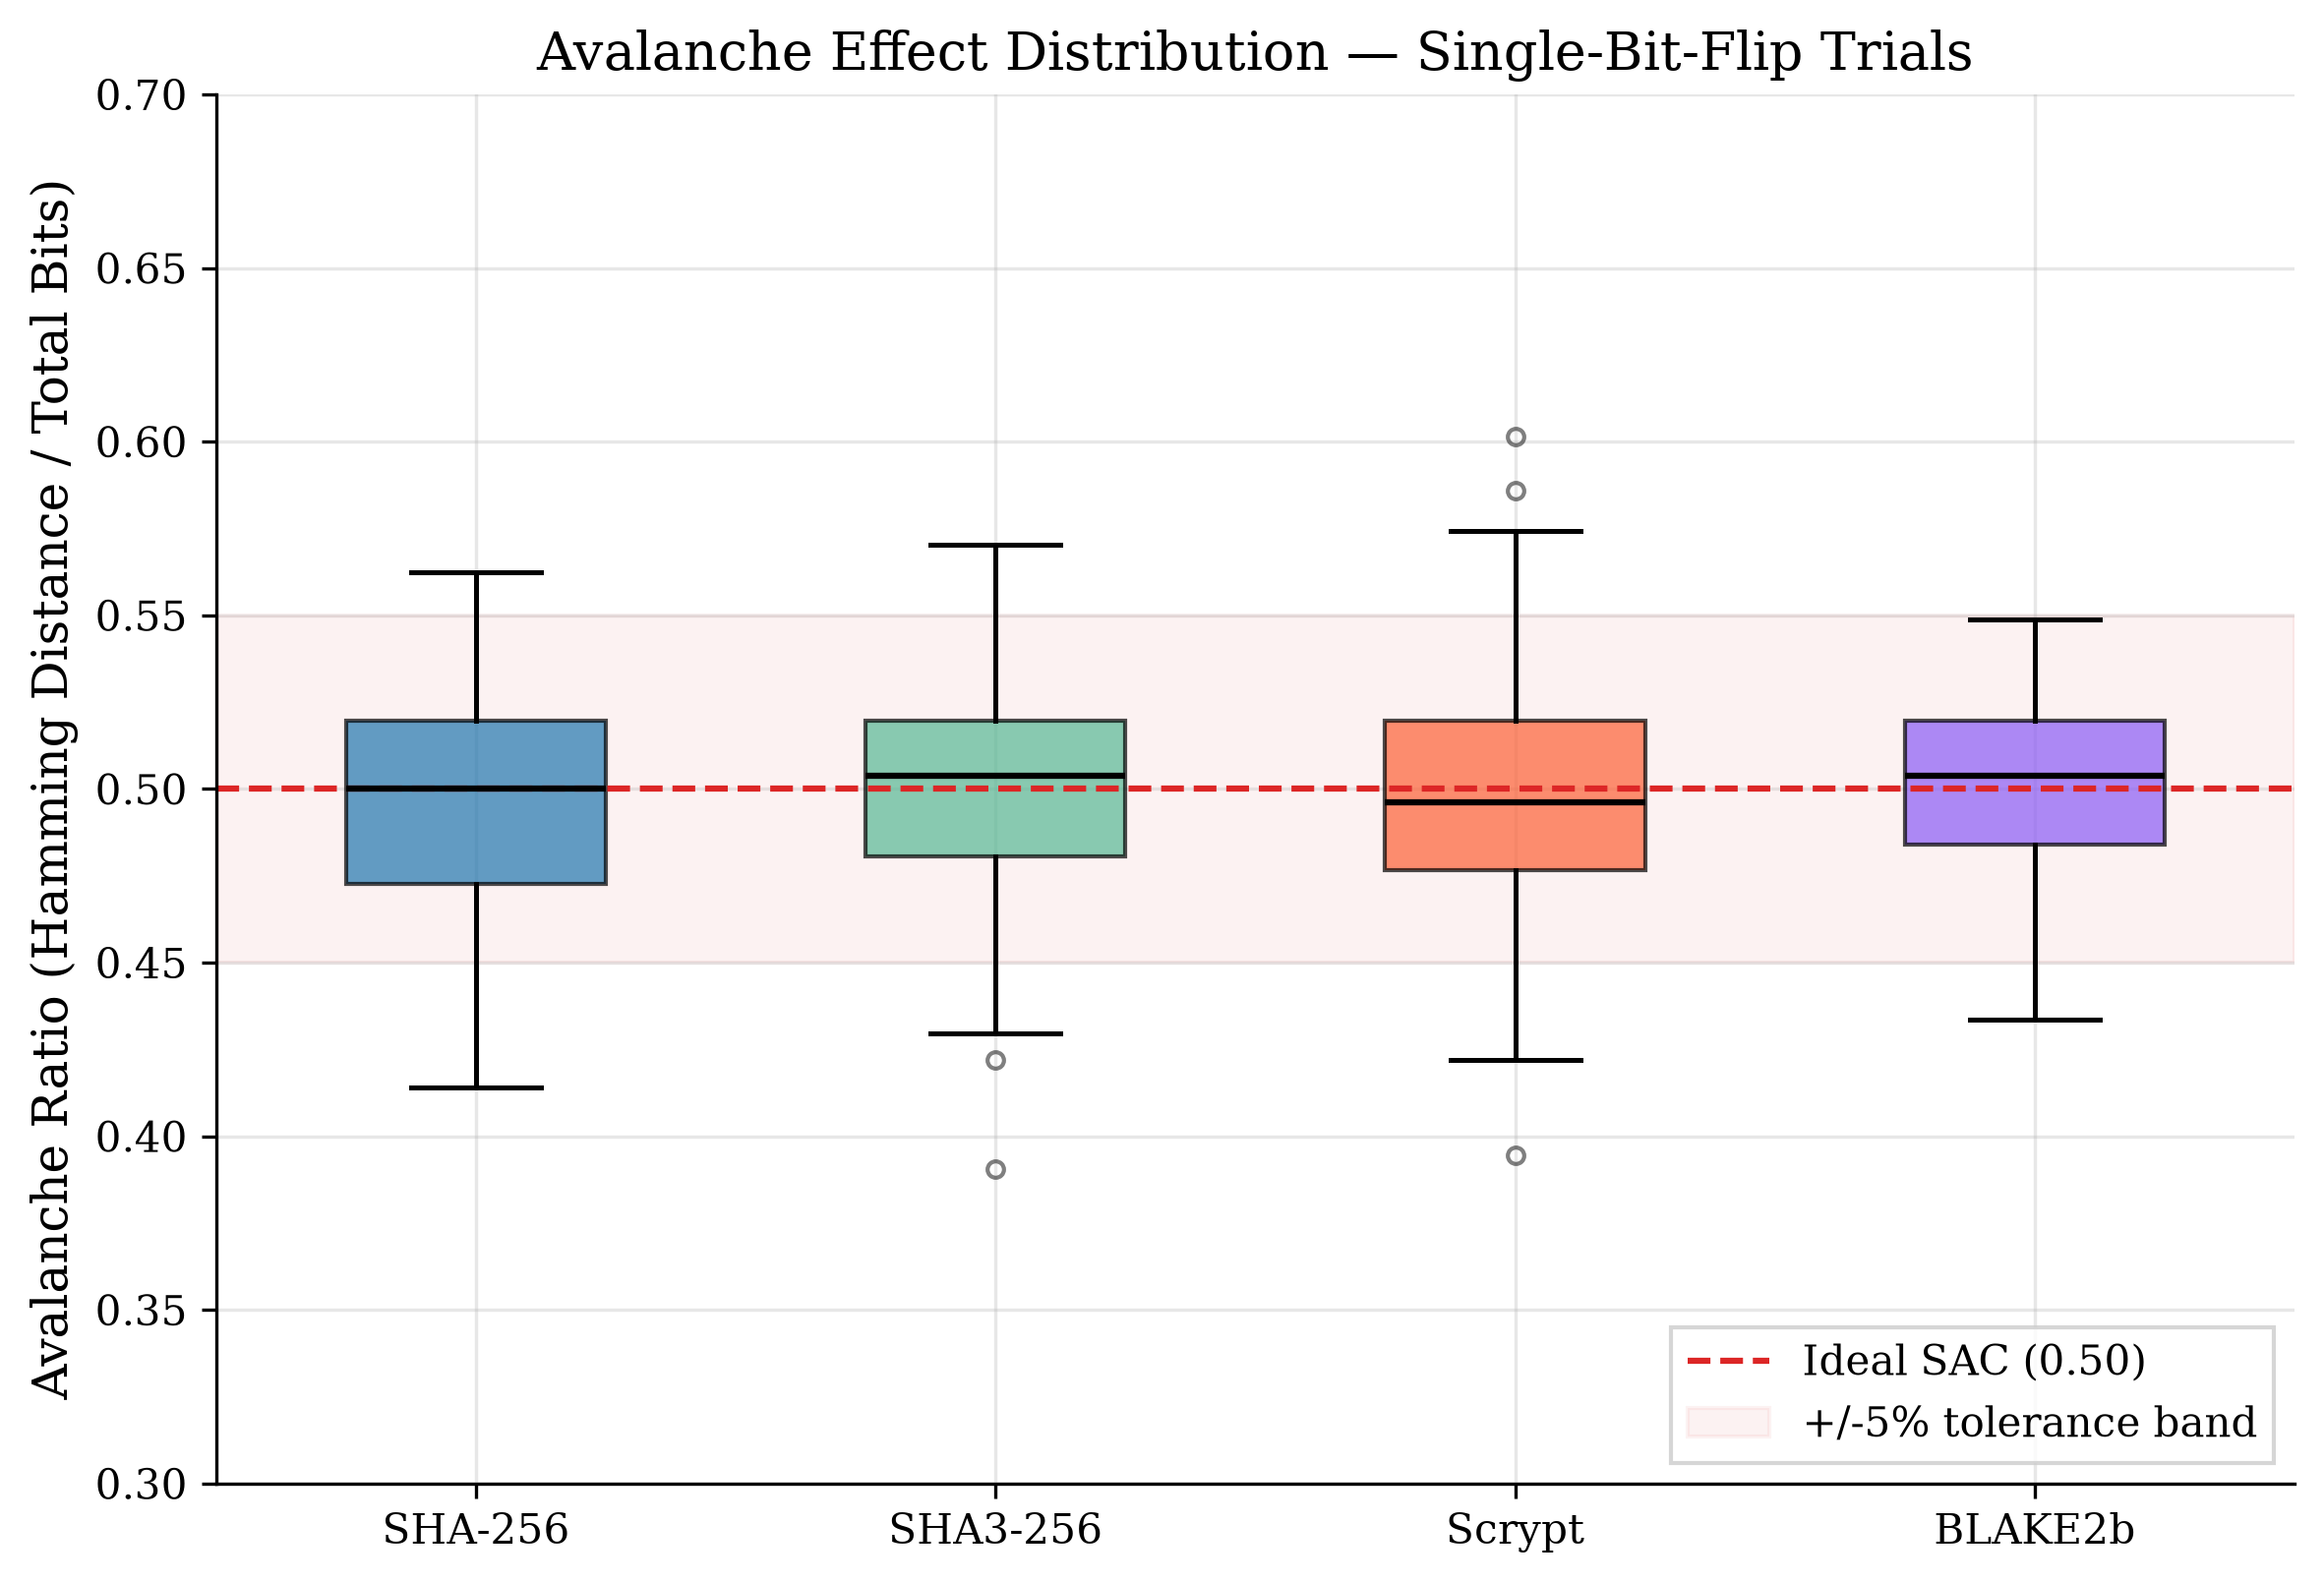
\includegraphics[width=0.88\linewidth]{figures/avalanche_distribution.png}
    \caption{Avalanche Effect distribution across 20 single-bit-flip trials. All algorithms adhere tightly to the 50\% theoretical SAC line within the $\pm 5\%$ tolerance band.}
    \label{fig:avalanche}
\end{figure}

The empirical SAC results are summarized in Table~\ref{tab:avalanche}. All four architectures exhibit a bit variance tightly centered near 50\%. This confirms that despite their vastly different internal designs, all four algorithms successfully scramble data to a degree that prevents attackers from guessing the input based on the output.

\begin{table}[H]
    \centering
    \caption{Strict Avalanche Criterion (SAC) Verification Across 20 Bit-Flip Trials}
    \label{tab:avalanche}
    \vspace{0.4em}
    \begin{tabular}{llcc}
        \toprule
        \textbf{Algorithm} & \textbf{Architecture} & \textbf{Digest Length} & \textbf{Mean Avalanche Ratio} \\
        \midrule
        SHA-256            & Merkle-Damg{\aa}rd    & 256 bits               & 49.61\%                       \\
        SHA3-256           & Sponge (Keccak)       & 256 bits               & 49.88\%                       \\
        Scrypt             & Memory-Hard PBKDF     & 256 bits               & 49.80\%                       \\
        BLAKE2b            & ARX                   & 512 bits               & 50.04\%                       \\
        \bottomrule
    \end{tabular}
\end{table}

\section{Memory Profiling \& Memory-Hardness Verification}
Next, we tested the economic defense mechanisms of the algorithms. By tracking the RAM allocated to the hashing process by the operating system, we can see if an algorithm is "memory-hard." Note that while our baseline throughput and avalanche benchmarks use Litecoin-style Scrypt parameters ($N=1024, r=1, p=1$), that baseline configuration only allocates $128 \times 1 \times 1024 = 128$~KiB of scratchpad memory, which OpenSSL allocates and frees faster than OS-level RSS polling can observe. Therefore, for the memory-hardness verification, we deliberately scaled Scrypt's cost parameters up to $N=32768, r=8, p=1$ ($128 \times 8 \times 32768 = 32.00$~MiB) to make the memory footprint macroscopically measurable. The results are illustrated in Figure~\ref{fig:memory} and quantified in Table~\ref{tab:memory}.

\begin{figure}[H]
    \centering
    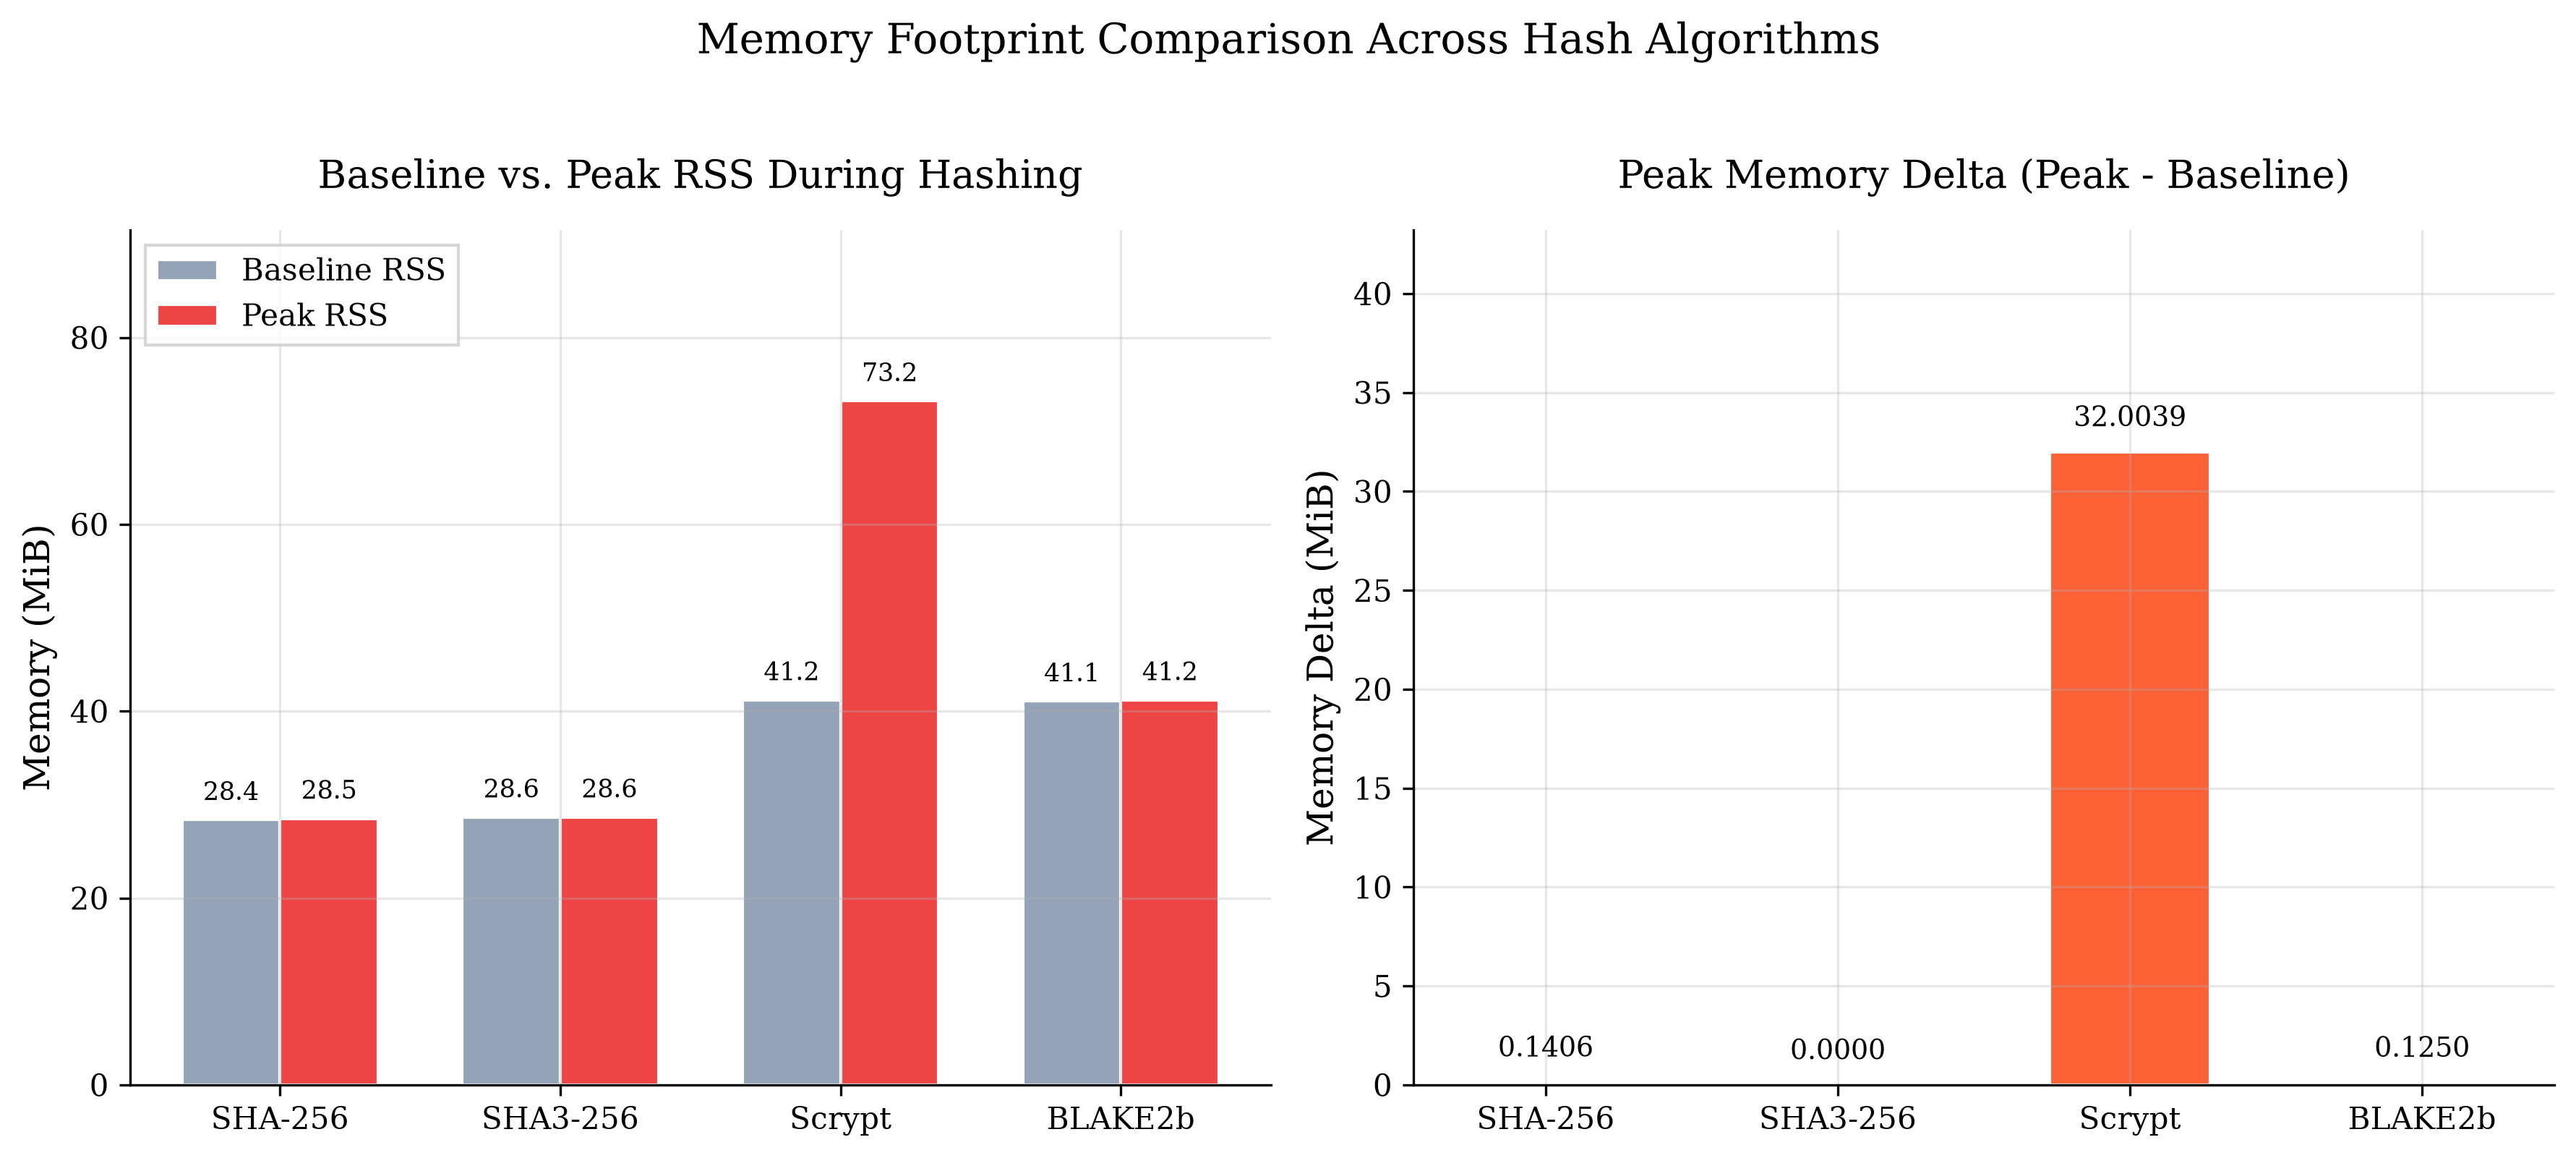
\includegraphics[width=0.92\linewidth]{figures/memory_consumption.png}
    \caption{System memory allocation profiles. Pure hash functions operate with negligible memory delta ($\le 0.15$~MiB), while Scrypt with scaled parameters ($N=32768, r=8, p=1$) enforces a 32.00~MiB allocation.}
    \label{fig:memory}
\end{figure}

\begin{table}[H]
    \centering
    \caption{Resident Set Size (RSS) Memory Profiling Summary}
    \label{tab:memory}
    \vspace{0.4em}
    \begin{tabularx}{\textwidth}{@{}l >{\raggedright\arraybackslash}X c c@{}}
        \toprule
        \textbf{Algorithm} & \textbf{Execution Mode}     & \textbf{Theoretical Allocation} & \textbf{Peak Memory $\Delta$ (MiB)} \\
        \midrule
        SHA-256            & Streaming (512-bit blocks)  & Negligible ($\sim 0$ B)         & 0.1406                              \\
        SHA3-256           & Streaming (1600-bit state)  & Negligible ($\sim 0$ B)         & 0.0000                              \\
        Scrypt             & Scaled ($N=32768, r=8$)     & 32.00 MiB                       & 32.0039                             \\
        BLAKE2b            & Streaming (128-byte blocks) & Negligible ($\sim 0$ B)         & 0.1250                              \\
        \bottomrule
    \end{tabularx}
\end{table}

The empirical measurements perfectly validate the theoretical claims:
\begin{itemize}
    \item \textbf{In-Register Streaming:} SHA-256, SHA3-256, and BLAKE2b process data in tiny, manageable blocks using the processor's ultra-fast internal registers. They do not need system RAM to function, resulting in a memory footprint of nearly zero ($\le 0.15$~MiB). This is exactly why ASICs can easily compute SHA-256.
    \item \textbf{Scrypt Memory-Hardness:} When we scaled Scrypt's difficulty parameters up ($N=32768, r=8, p=1$), it forcibly claimed \textbf{32.00~MiB} of system memory to execute a single hash. If an ASIC manufacturer wanted to build a chip that calculates one million Scrypt hashes a second, they would have to physically wire 32 Terabytes of high-speed RAM directly onto the silicon---an economically impossible task. This proves exactly how Scrypt keeps Litecoin mining decentralized.
\end{itemize}

\section{Throughput, Latency, and Hardware Dynamics}
Finally, we benchmarked pure speed by digesting payloads scaling from 1~KB to 100~MB. To ensure that hardware-specific capabilities (like Intel's SHA-NI) did not skew the dataset, Node A and Node B were benchmarked and plotted entirely independently. For these timing trials, Scrypt was evaluated using its baseline parameters ($N=1024, r=1, p=1$) rather than the 32~MiB memory-profiling configuration so that multi-payload timing runs remain computationally tractable. The throughput profiles are presented in Figure~\ref{fig:throughput} and summarized in Table~\ref{tab:throughput}.

\begin{figure}[H]
    \centering
    % NOTE: Update these paths if plotting side-by-side or stacked
    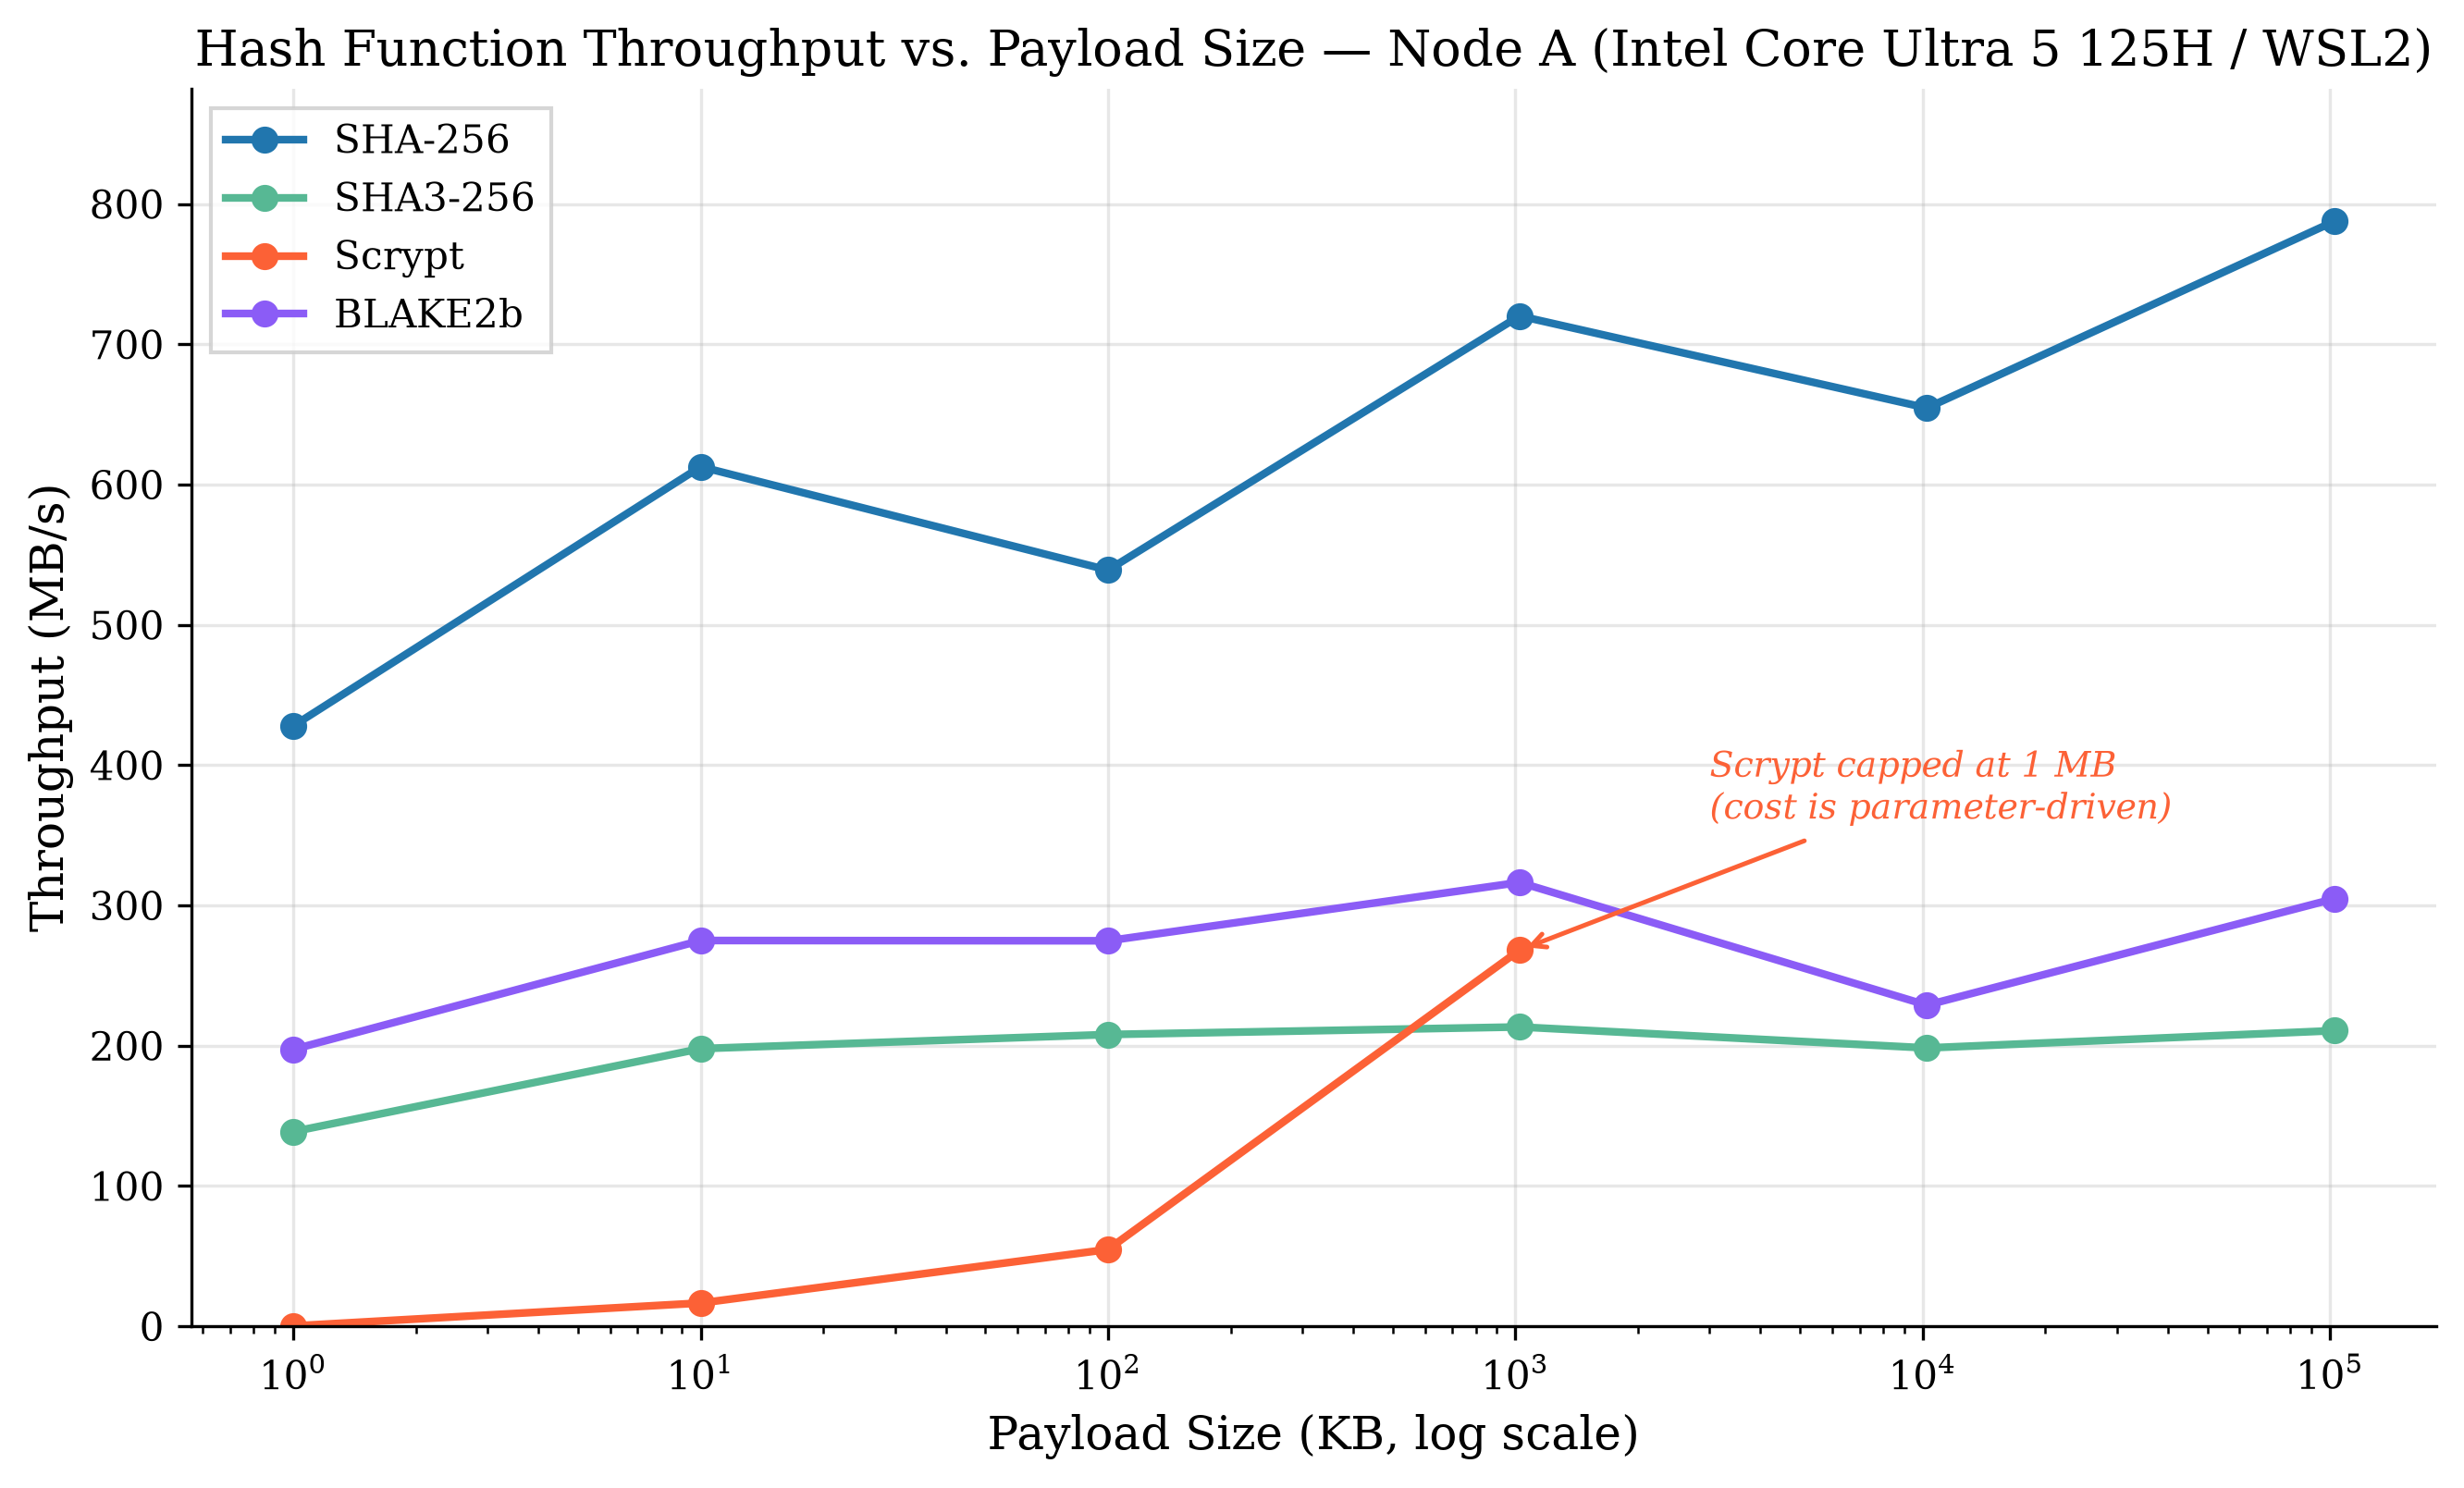
\includegraphics[width=0.48\linewidth]{figures/throughput_node_a.png}
    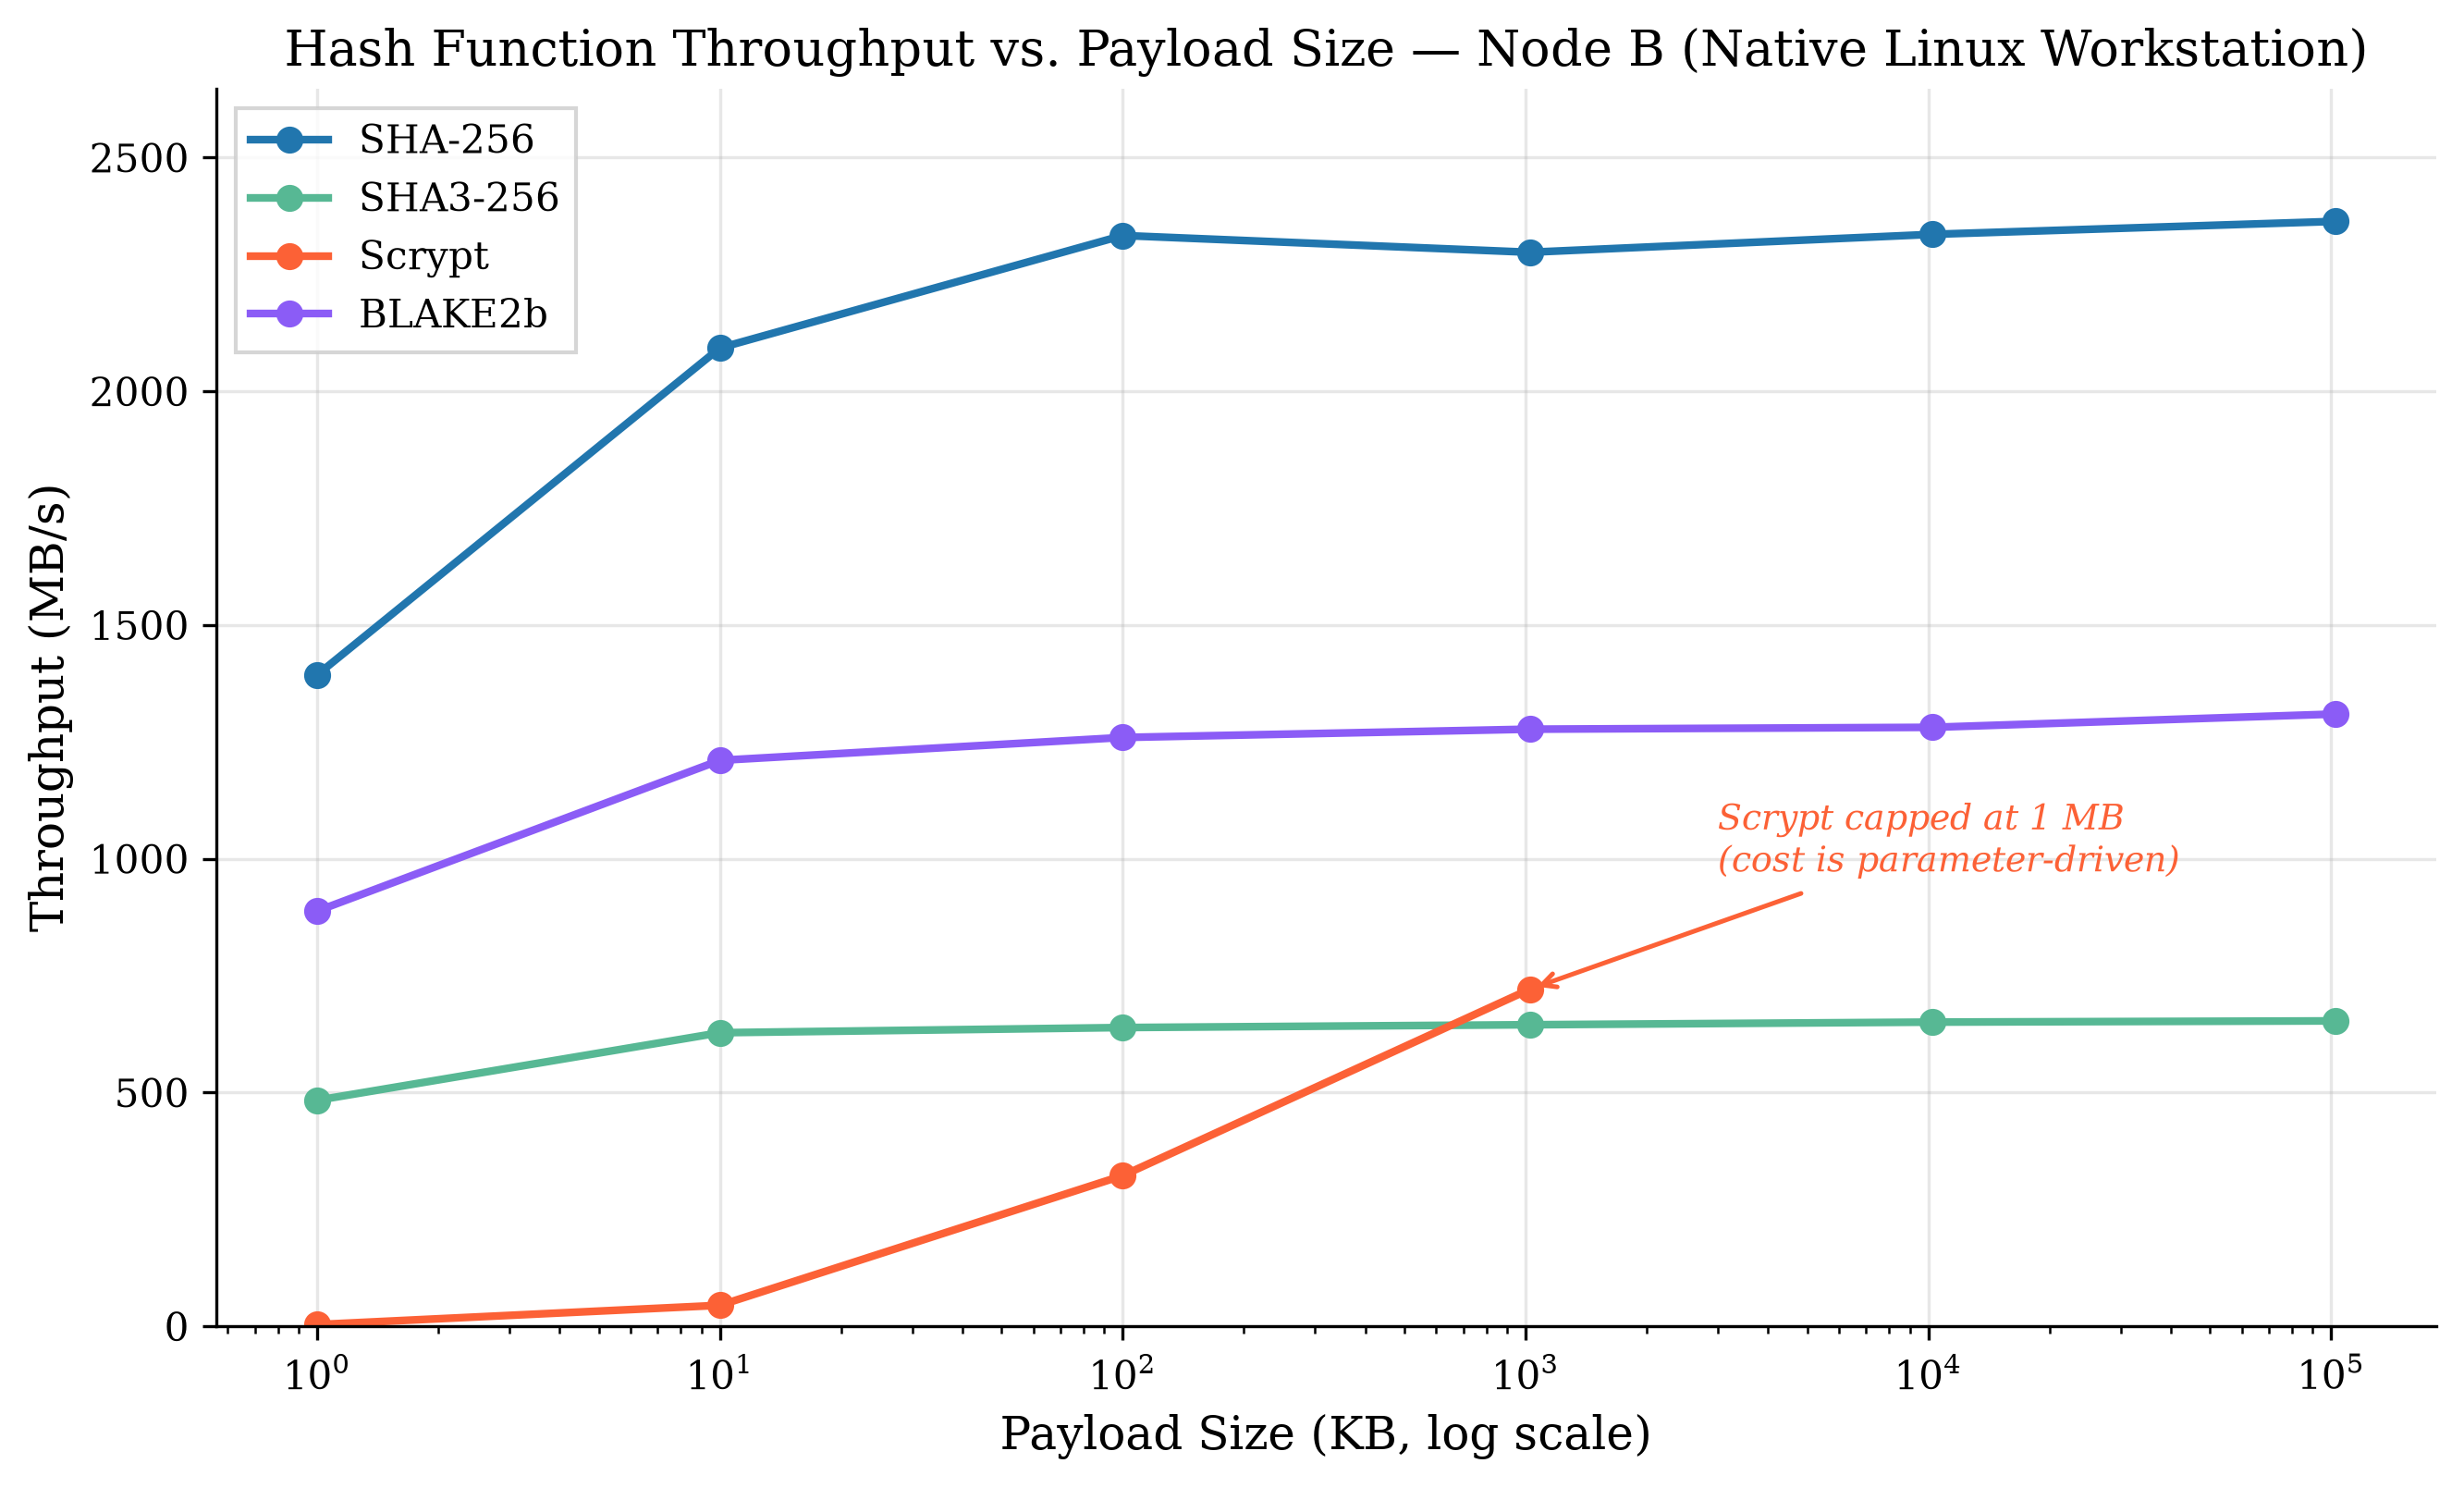
\includegraphics[width=0.48\linewidth]{figures/throughput_node_b.png}
    \caption{Independent Throughput profiles for Node A (Intel Core Ultra 5, left) and Node B (AMD Ryzen 7, right).}
    \label{fig:throughput}
\end{figure}

\begin{table}[H]
    \centering
    \caption{Independent Peak Throughput Performance Across Nodes}
    \label{tab:throughput}
    \vspace{0.4em}
    \begin{tabularx}{\textwidth}{@{}l l c c >{\raggedright\arraybackslash}X@{}}
        \toprule
        \textbf{Algorithm} & \textbf{Architecture} & \textbf{Node A Peak} & \textbf{Node B Peak} & \textbf{Primary Performance Factor} \\
        \midrule
        SHA-256            & Merkle-Damg{\aa}rd    & 787.67 MB/s          & 2363.55 MB/s         & Hardware acceleration availability  \\
        BLAKE2b            & ARX                   & 316.44 MB/s          & 1309.68 MB/s         & 64-bit software pipeline speed      \\
        Scrypt             & Memory-Hard PBKDF     & 268.12 MB/s          & 720.88 MB/s          & Constant setup cost amortization    \\
        SHA3-256           & Sponge (Keccak)       & 213.39 MB/s          & 653.28 MB/s          & Permutation state overhead          \\
        \bottomrule
    \end{tabularx}
\end{table}

Isolating the hardware profiles highlights three key observations about how these algorithms perform in practice:
\begin{enumerate}
    \item \textbf{Hardware Acceleration Defeats Software Design:} The literature survey states that BLAKE2b was meticulously designed to be the fastest software algorithm. However, on modern processors equipped with dedicated SHA Extensions (SHA-NI), SHA-256 completely dominates software-bound algorithms (peaking at 787.67~MB/s on Node A and 2363.55~MB/s on Node B, compared to 316.44~MB/s and 1309.68~MB/s for BLAKE2b). Dedicated silicon instructions easily outpace even the most optimized general-purpose software routines.
    \item \textbf{The Cost of Security:} Across both nodes, SHA3-256 remains the slowest pure hash algorithm (peaking at 213.39~MB/s on Node A and 653.28~MB/s on Node B). This illustrates the direct computational cost of Ethereum's choice to manipulate the massive 1600-bit Sponge state to prevent length-extension attacks. Higher security margins demand more mathematical work per byte.
    \item \textbf{Throughput Saturation and Scaling:} For the streaming hash functions (SHA-256, BLAKE2b, and SHA3-256), throughput rises sharply from 1~KB to a saturation point around 100~KB ($10^2$~KB), where initial function-call overhead is fully amortized. Beyond 100~KB, Node B maintains a smooth, flat plateau all the way to 100~MB. On Node A, this plateau looks slightly uneven because it runs inside a virtualized environment (WSL2) on a hybrid processor, where background OS scheduling and core switching introduce minor fluctuations. Conversely, even under its baseline configuration ($N=1024, r=1, p=1$), Scrypt's runtime is dominated by its fixed PBKDF iteration cost; it exhibits near-zero throughput at 1~KB and only reaches high MB/s figures at 1~MB once its constant setup cost is spread across a large enough payload.
\end{enumerate}


\chapter{Work Yet to be Completed}

While Phase 1 successfully profiled the integrity pillar via hashing primitives, Phase 2 will shift focus to the authentication and non-repudiation pillars by evaluating public-key digital signatures:

\begin{enumerate}
    \item \textbf{Signature Algorithm Selection:} Profile standard modular exponentiation schemes alongside modern elliptic curves used in high-volume networks.
    \item \textbf{Computational Asymmetry Evaluation:} In blockchain nodes, transaction volume requires signature verification to be significantly faster than signature generation. We will benchmark the temporal asymmetry between key generation, signing, and verification latency.
    \item \textbf{Storage and Serialization Footprints:} Measure the wire-protocol byte footprint of raw public keys and signatures to quantify storage scalability across different mathematical approaches.
    \item \textbf{Signature Aggregation Analysis:} Analyze how advanced aggregation primitives reduce validator verification overhead by batching multiple signatures into a single validation pass.
\end{enumerate}


% =============================================================================
% BIBLIOGRAPHY
% =============================================================================
\begin{thebibliography}{00}
    \addcontentsline{toc}{chapter}{References}

    \bibitem{schneier1996applied}
    B.~Schneier, \emph{Applied Cryptography: Protocols, Algorithms, and Source Code in C}, 2nd~ed. New York, NY: John Wiley \& Sons, 1996.

    \bibitem{paar2024understanding}
    C.~Paar, J.~Pelzl, and T.~G{\"u}neysu, \emph{Understanding Cryptography: A Textbook for Students and Practitioners}, 2nd~ed. Berlin, Heidelberg: Springer, 2024.

    \bibitem{nakamoto2008bitcoin}
    S.~Nakamoto, ``Bitcoin: A Peer-to-Peer Electronic Cash System,'' White Paper, 2008. [Online]. Available: \url{https://bitcoin.org/bitcoin.pdf}

    \bibitem{wood2014ethereum}
    G.~Wood, ``Ethereum: A Secure Decentralised Generalised Transaction Ledger,'' Ethereum Project Yellow Paper, 2014.

    \bibitem{bertoni2013keccak}
    G.~Bertoni, J.~Daemen, M.~Peeters, and G.~Van Assche, ``Keccak,'' in \emph{Advances in Cryptology -- EUROCRYPT 2013}, Lecture Notes in Computer Science, vol.~7881. Berlin, Heidelberg: Springer, 2013, pp.~313--314.

    \bibitem{percival2009scrypt}
    C.~Percival, ``Stronger Key Derivation Via Sequential Memory-Hard Functions,'' in \emph{Proceedings of BSDCan 2009}, Ottawa, Canada, May 2009.

    \bibitem{aumasson2013blake2}
    J.-P.~Aumasson, S.~Neves, Z.~Wilcox-O'Hearn, and C.~Winnerlein, ``BLAKE2: Simpler, smaller, fast as MD5,'' in \emph{Applied Cryptography and Network Security (ACNS 2013)}, Lecture Notes in Computer Science, vol.~7954. Berlin, Heidelberg: Springer, 2013, pp.~119--135.

\end{thebibliography}

\end{document}